%interaction with it, programs, geometry represenations, datastructures, formats etc., maybe even history if we're overkill
\subsection{History of CAD}
Computer aided design (short: CAD) refers to the process of designing a product using a computer system. Before CAD applications were used, products were constructed using a sketch board. It was a challenge to incorporate changes in the construction drafts as well as to keep documentations up to date; hence, it was no surprise that CAD systems spread rapidly across all design development branches. Computer aided design is now irreplaceable used in architecture, mechanical, electrical and civil engineering.

Depending on the discipline different requirements are set on the virtual model. One may imagine that in a civil engineering model of a building a 2D floor plan is often sufficient; however in the design of a mechanical motor a 3D model is always necessary. Given these circumstances, various CAD software bundles evolved in the different disciplines with completely different modelling approaches. Besides the geometry representation additional parameters, such as material properties or manufacturing information, are stored. In order to move between different data structures standardized exchange interfaces are commonly used.
\subsection{Geometry representations}
In general, two different ways of describing a geometry are used in CAD systems: constructive solid geometry consisting of a set of primitive forms or storing the boundary of a part assuming that the interior is filled (BREP). Other approaches, such as a complete voxelised geometry are not common due to extensive memory consumption.
\subsubsection{Constructive solid geometry}
\begin{figure}
\centering
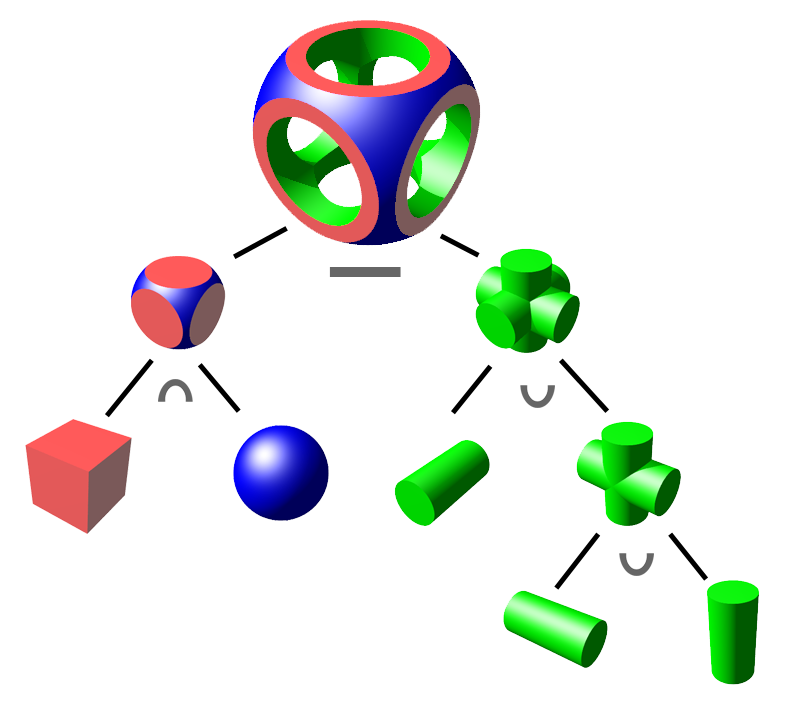
\includegraphics[width=0.5\textwidth]{Pictures/Csg_tree.png}
\caption{CSG object tree}
\label{fig:csg_tree}
\end{figure}
One way of representing a geometry in CAD is the approach of \emph{constructive solid geometry} (short: CSG). The basic idea is to start from a set of primitives, e.g. a sphere, cylinder and cube. Basic Boolean operations link these primitives towards a complex geometry. This procedure can be seen in figure \ref{fig:csg_tree}.

Key advantages of this format is the precise representation using very few storage memory. However, not all desired forms can be represented by CSG and hence, a second type of geometry description is needed. 
\subsubsection{Boundary representation}
A different kind of modelling approach is the so-called \emph{boundary representation}. Instead of storing the geometry information at every single point, \emph{BREP} formats only save the boundary surface of the body. The interior is assumed to be uniformly filled. Especially in big geometries this approach simplifies the model immensely to an extend that amounts of data are better to handle. Surfaces can be for example stored as a set of triangles (see later STL files) or in NURBS patches.
Furthermore, holes in the body are possible by saving the specifying the surface normal of the respective boundary. 

By the boundary representation arbitrary geometries can be created. Data amounts to fulfill a certain precision are larger than by the csg representation, but BREP files are usually easier to work with. Keep in mind that non-physical geometries can result from BREP formats through a not closed surface.
\subsection{Data exchange file formats}
CAD software programs usually use own data formats; in order to exchange models standardized interface formats are developed. Geometry information of the model is compressed to certain geometry descriptions and other programs can create a new model in its own file type by this information. Transferring additional information, such as material properties or manufacturing information is general a difficult task or prohibited by the exchange file format. A few common exchange file types are described in the following.
\subsubsection{STL file format}
The \emph{ST}ereo\emph{L}ithography file format describes the model only by its boundary (BREP); thus, only geometric information can be transferred. 

The idea behind the STL files is simple; the geometric model is discretized into a cloud of points. In three dimensions  three of these vertices form a triangle; this is done for all vertices and hence the connected surface of triangles describes the surface of the body (BREP). This procedure is shown in figure \ref{fig:STL} for a two dimensional circle.  
\begin{figure}
\centering
   \scalebox{0.4}{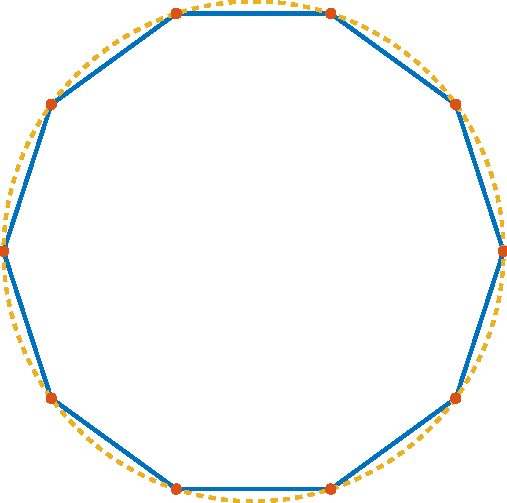
\includegraphics{Pictures/STL.pdf}}\\
   \caption{STL discretization for a circle}
   \label{fig:STL}
\end{figure}
In two dimensions the mentioned triangles are lines. The advantages and disadvantages of this approach becomes clear: It can be applied to an arbitrary geometry, but accuracy causes difficulties. In order to to transfer high precision geometries many vertices are necessary. This will result in big files; nevertheless, a precise circle can never be represented. 

ASCII STL files begin with a name and data on the triangles are constructed as follows: 
\begin{itemize}
\item a facet normal pointing outward
\item a loop of vertex coordinates
\end{itemize}
Note that no additional information such as material properties can be transferred through STL files. 
\subsubsection{IGES file format}
To overcome these issues with there exist also more elaborate exchange formats that save e.g. a circle as a parameter where no discretisation step is involved. Also, the possibility of passing additional parameter information is required by certain users. Popular file types that offer these two functionalities are STEP and IGES files. 

The IGES file format contains five different sections; a Start, Global, Directory Entry, Parameter Data, and Terminate section. The start and global section are used for naming and part information. In the directory entry additional information like the node color is saved. The parameter data section is used for storing the coordinate points and the terminate section signals the end of the file. 
